\subsection{概述}
\label{subsec:sgxdedup-arch}

\begin{figure}[t]
\centering
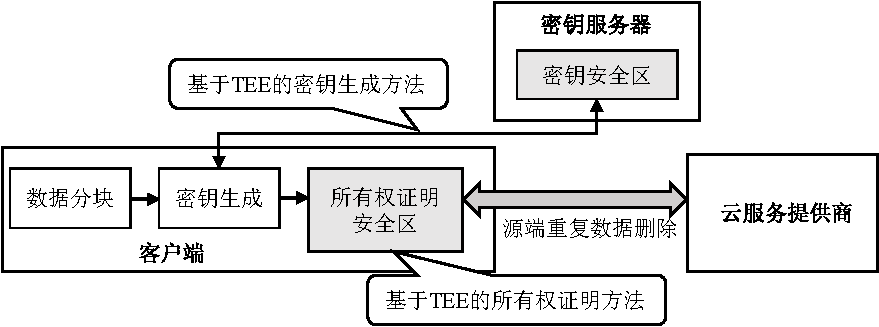
\includegraphics[width=\textwidth]{pic/sgxdedup/sgxdedup-arch.pdf}
\caption{\sysnameS 系统架构概述:\sysnameS 在密钥服务器和每个客户端中分别部署了密钥安全区和所有权证明安全区。}
\label{fig:sgxdedup-overview}
\vspace{-3pt}
\end{figure}

\paragraph*{架构:} 图~\ref{fig:sgxdedup-overview} 展示了\sysnameS 的系统架构,其中引入了两个安全区:\textit{密钥安全区(Key Enclave)} 和 \textit{所有权证明安全区(PoW Enclave)}。 

\begin{figure}[!htb]
  \centering
  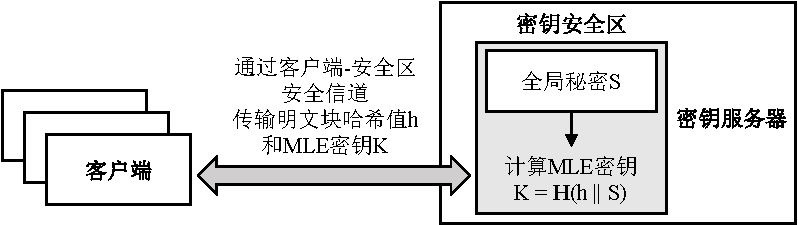
\includegraphics[width=\textwidth]{pic/sgxdedup/key-enclave.pdf}
  \caption{\sysnameS 系统架构: 密钥安全区}
  \label{fig:sgxdedup-overview-key}
  \vspace{-3pt}
\end{figure}


\sysnameS 在密钥服务器中部署一个\textit{密钥安全区(Key Enclave)},以管理和保护服务器辅助消息锁加密所需的的全局秘密,使其免受受损密钥服务器的侵害。要执行 消息锁加密(MLE) 密钥生成,密钥安全区和客户端都首先基于共享 \textit{盲密钥} 建立一个安全通道(有关如何形成盲密钥的详细信息,请参阅 \S\ref{subsec:sgxdedup-key-management})。然后客户端通过安全通道提交明文数据块的指纹。密钥安全区计算 消息锁加密(MLE) 密钥作为全局秘密和指纹的加密哈希。它通过安全通道返回 消息锁加密(MLE) 密钥。

密钥安全区有利于性能和安全性。它避免了在 消息锁加密(MLE) 密钥生成期间服务器辅助 消息锁加密(MLE) 的昂贵的 OPRF 协议 \cite{bellare2013DupLESS}。此外,它通过基于共享盲密钥的安全通道保护指纹和 消息锁加密(MLE) 密钥,这样密钥服务器就无法从 消息锁加密(MLE) 密钥生成过程中学习任何信息。此外,它保护安全区内存中的全局秘密,即使密钥服务器受到威胁也能保持安全性(请注意,当密钥服务器受到威胁时,原始服务器辅助 消息锁加密(MLE) 的安全性会降低;请参阅 \S\ref{subsec:sgxdedup-problem})。
  w
\begin{figure}[!htb]
  \centering
  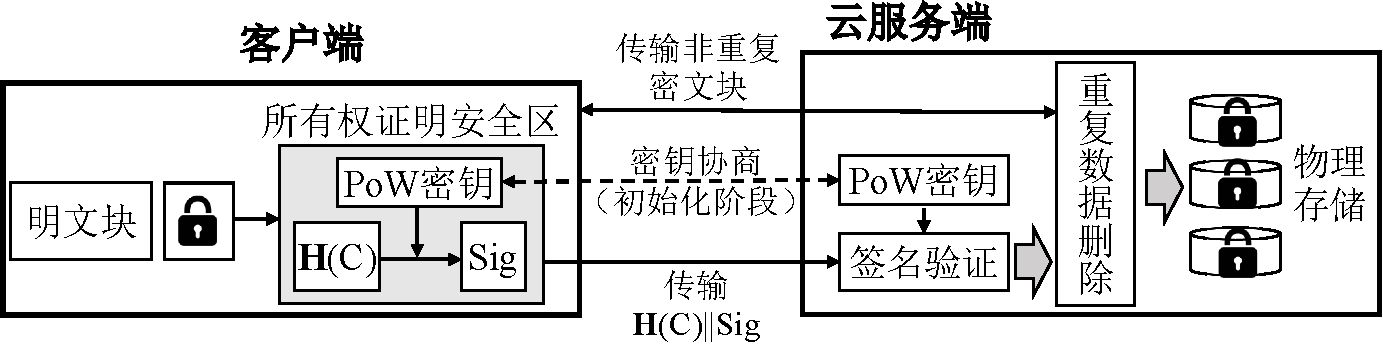
\includegraphics[width=\textwidth]{pic/sgxdedup/pow.pdf}
  \caption{\sysnameS 系统架构: 所有权证明安全区}
  \label{fig:sgxdedup-overview-pow}
  \vspace{-3pt}
\end{figure}

\sysnameS 在每个客户端中部署一个所有权证明安全区,以证明源端重复数据删除中密文数据块的真实性。所有权证明安全区首先与云建立一个共享的 \textit{PoW Key}(本文目前使用 Diffie-Hellman 密钥交换 (DHKE) 实现密钥协商;参见 \S\ref{sec:sgxdedup-implementation})。生成 消息锁加密(MLE) 密钥后,客户端将每个明文数据块加密为密文数据块。 所有权证明安全区将密文数据块作为输入,计算相应的指纹,并使用与云共享的PoW Key创建指纹的签名。然后客户端将指纹和签名上传到云端。云端根据对应的签名和PoW Key验证指纹的真实性。只有当指纹被认证时,云才会继续检查指纹是否对应于任何已经存储的重复密文数据块。请注意,本文验证客户端对密文数据块的所有权而不是明文的所有权(例如,\cite{halevi11}),以保护原始信息不被云端访问。确保密文数据块的所有权足以保证安全,因为 消息锁加密(MLE) 应用一对一的映射,并且密文数据块的所有权与对应的明文数据块的所有权一致。

所有权证明安全区再次有利于性能和安全性。它避免了加密 PoW 结构的计算开销。它还保护重复数据删除模式免受恶意客户端的攻击,因为模式仅在经过身份验证的指纹后才会返回。

请注意,先前的研究 \cite{kim2019ShieldStore,fuhry20,djoko2019NEXUS} 在安全区内执行密钥生成和加密,而本文选择在未受保护的内存中执行加密。主要原因是原始明文数据块和加密过程都位于客户端内。将加密过程移动到安全区并不能提高安全性,因为妥协的客户端也可以访问其明文数据块,但它会增加安全区的大量计算开销。

\begin{table}[t]
\small
\centering
\begin{tabular}{ccc}
\toprule
{\bf 所属安全区} & {\bf ECall名称} & {\bf 描述}\\ 
\midrule
\multirow{5}{*}{\bf 密钥安全区}
& \textit{ Secret generation} & 产生全局秘密 
(\S\ref{subsec:sgxdedup-enclave-management}) \\
& \textit{ Rekeying} & 更新盲密钥 
(\S\ref{subsec:sgxdedup-key-management}) \\
& \textit{ Nonce checking} & 检查nonce合规性 
(\S\ref{subsec:sgxdedup-encryption}) \\
& \textit{ Key generation} & 产生消息锁加密(MLE)密钥 (\S\ref{subsec:sgxdedup-encryption}) \\
& \textit{ Mask generation} & 生成加密掩码 (\S\ref{subsec:sgxdedup-encryption}) \\
\hline
\multirow{3}{*}{\bf 所有权证明安全区}
& \textit{ Key unsealing} & 从磁盘解封所有权证明密钥 (\S\ref{subsec:sgxdedup-enclave-management}) \\
& \textit{ Key sealing} & 密封所有权证明密钥至磁盘 (\S\ref{subsec:sgxdedup-enclave-management}) \\
& \textit{ Proof generation} & 签名密文数据块对应的指纹 
(\S\ref{sec:sgxdedup-implementation}) \\
\bottomrule
\end{tabular}
\vspace{-6pt}
\caption{\sysnameS 中的Ecall(安全区调用)}
\label{tab:sgxdedup-ecall}
\vspace{-3pt}
\end{table}

\paragraph*{问题。} 有效地​​实现基于 SGX 的加密后重复数据删除并非易事,因为本文需要减轻 SGX 的潜在性能开销,否则会抵消整体性能优势。在这里,本文提出了三个问题,本文基于一套用于密钥安全区和所有全证明安全区 (Table~\ref{tab:sgxdedup-ecall}) 的 ECall 来解决这些问题。

\begin{itemize}[leftmargin=*]
\item 如何安全有效地引导安全区? (\S\ref{subsec:sgxdedup-enclave-management})
  密钥安全区维护全局秘密。在开始时将全局秘密安全地引导到密钥安全区中至关重要。此外,所有权证明安全区与客户端紧密绑定。它应该在客户端在线访问云时引导,并在客户端退出时以安全有效的方式终止。
\item 密钥安全区和每个客户端应该如何建立安全通道? (\S\ref{subsec:sgxdedup-key-management})
  每个客户端都基于共享的盲密钥与密钥安全区进行安全通信,以便生成必要的 消息锁加密(MLE) 密钥来保护外包块。由于客户端可能加入或退出云订阅组,盲密钥不仅要高效建立,而且可以更新以进行动态客户端认证。
\item 密钥安全区应该如何减少管理客户端安全通道的计算开销? (\S\ref{subsec:sgxdedup-encryption})
  在每个安全通道中(在密钥安全区和每个客户端之间),密钥安全区解密请求指纹并加密生成的 消息锁加密(MLE) 密钥。它的计算复杂度随着指纹数量和连接客户端的数量而增加。
\end{itemize}
